% This LaTeX document needs to be compiled with XeLaTeX.
\documentclass[10pt]{article}
\usepackage[utf8]{inputenc}
\usepackage{amsmath}
\usepackage{amsfonts}
\usepackage{amssymb}
\usepackage[version=4]{mhchem}
\usepackage{stmaryrd}
\usepackage{graphicx}
\usepackage[export]{adjustbox}
\graphicspath{ {./images/} }
\usepackage[fallback]{xeCJK}
\usepackage{polyglossia}
\usepackage{fontspec}
\setCJKmainfont{Noto Serif CJK JP}

\setmainlanguage{polish}
\setmainfont{CMU Serif}

\title{LIGA MATEMATYCZNA \\
 PÓŁFINAモ \\
 16 lutego 2012 \\
 GIMNAZJUM }

\author{}
\date{}


\begin{document}
\maketitle
\section*{ZADANIE 1.}
Uzasadnij, że suma czterech kolejnych liczb naturalnych nieparzystych nie może być liczbą pierwsza.

\section*{ZADANIE 2.}
Wykaż, że \(\sqrt{17-12 \sqrt{2}}+\sqrt{17+12 \sqrt{2}}\) jest liczbą całkowitą.

\section*{ZADANIE 3.}
W każdym kroku wykonujemy na liczbie jedną z operacji (w dowolnej kolejności):

\begin{itemize}
  \item podwajamy liczbę;
  \item skreślamy jej ostatnią cyfrę.
\end{itemize}

Czy w taki sposób po skończonej ilości operacji można z liczby 378 uzyskać 16?

\section*{ZADANIE 4.}
Oblicz \(1+2-3-4+5+6-7-8+9+10-\ldots-2011-2012+2013+2014\).

\section*{ZADANIE 5.}
Na prostokątnej tacy Asia układała dwie kwadratowe serwetki o polu \(900 \mathrm{~cm}^{2}\) każda. Gdy ułożyła je tak, jak na pierwszym rysunku, to zachodziły na siebie na obszarze o polu \(300 \mathrm{~cm}^{2}\), gdy tak, jak na drugim rysunku, to wspólny obszar miał \(750 \mathrm{~cm}^{2}\). Jakie pole będzie miał wspólny obszar obu serwetek, gdy Asia ułoży je w sposób przedstawiony na trzecim rysunku?\\
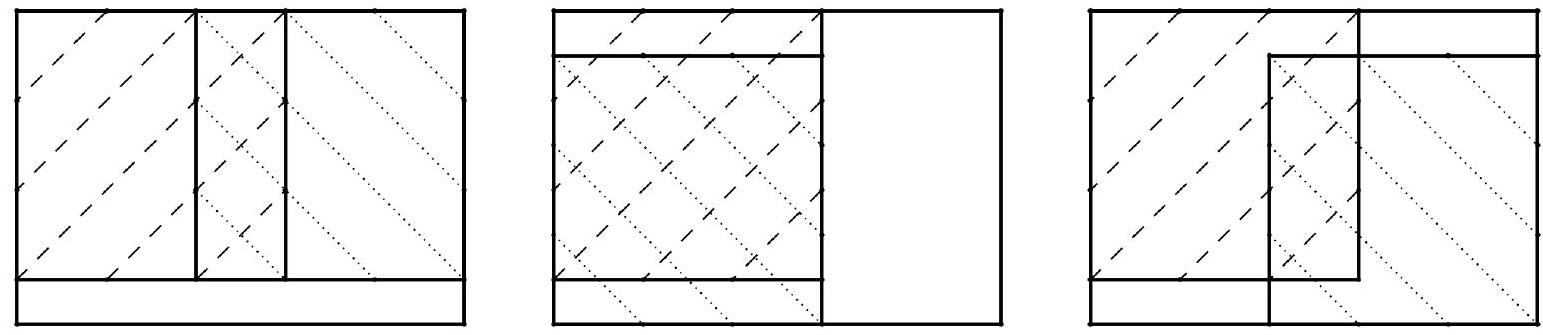
\includegraphics[max width=\textwidth, center]{2024_11_21_4688d04d730bb3126de2g-1}


\end{document}